\documentclass[twoside]{book}

% Packages required by doxygen
\usepackage{fixltx2e}
\usepackage{calc}
\usepackage{doxygen}
\usepackage[export]{adjustbox} % also loads graphicx
\usepackage{graphicx}
\usepackage[utf8]{inputenc}
\usepackage{makeidx}
\usepackage{multicol}
\usepackage{multirow}
\PassOptionsToPackage{warn}{textcomp}
\usepackage{textcomp}
\usepackage[nointegrals]{wasysym}
\usepackage[table]{xcolor}

% Font selection
\usepackage[T1]{fontenc}
\usepackage[scaled=.90]{helvet}
\usepackage{courier}
\usepackage{amssymb}
\usepackage{sectsty}
\renewcommand{\familydefault}{\sfdefault}
\allsectionsfont{%
  \fontseries{bc}\selectfont%
  \color{darkgray}%
}
\renewcommand{\DoxyLabelFont}{%
  \fontseries{bc}\selectfont%
  \color{darkgray}%
}
\newcommand{\+}{\discretionary{\mbox{\scriptsize$\hookleftarrow$}}{}{}}

% Page & text layout
\usepackage{geometry}
\geometry{%
  a4paper,%
  top=2.5cm,%
  bottom=2.5cm,%
  left=2.5cm,%
  right=2.5cm%
}
\tolerance=750
\hfuzz=15pt
\hbadness=750
\setlength{\emergencystretch}{15pt}
\setlength{\parindent}{0cm}
\setlength{\parskip}{3ex plus 2ex minus 2ex}
\makeatletter
\renewcommand{\paragraph}{%
  \@startsection{paragraph}{4}{0ex}{-1.0ex}{1.0ex}{%
    \normalfont\normalsize\bfseries\SS@parafont%
  }%
}
\renewcommand{\subparagraph}{%
  \@startsection{subparagraph}{5}{0ex}{-1.0ex}{1.0ex}{%
    \normalfont\normalsize\bfseries\SS@subparafont%
  }%
}
\makeatother

% Headers & footers
\usepackage{fancyhdr}
\pagestyle{fancyplain}
\fancyhead[LE]{\fancyplain{}{\bfseries\thepage}}
\fancyhead[CE]{\fancyplain{}{}}
\fancyhead[RE]{\fancyplain{}{\bfseries\leftmark}}
\fancyhead[LO]{\fancyplain{}{\bfseries\rightmark}}
\fancyhead[CO]{\fancyplain{}{}}
\fancyhead[RO]{\fancyplain{}{\bfseries\thepage}}
\fancyfoot[LE]{\fancyplain{}{}}
\fancyfoot[CE]{\fancyplain{}{}}
\fancyfoot[RE]{\fancyplain{}{\bfseries\scriptsize Generated by Doxygen }}
\fancyfoot[LO]{\fancyplain{}{\bfseries\scriptsize Generated by Doxygen }}
\fancyfoot[CO]{\fancyplain{}{}}
\fancyfoot[RO]{\fancyplain{}{}}
\renewcommand{\footrulewidth}{0.4pt}
\renewcommand{\chaptermark}[1]{%
  \markboth{#1}{}%
}
\renewcommand{\sectionmark}[1]{%
  \markright{\thesection\ #1}%
}

% Indices & bibliography
\usepackage{natbib}
\usepackage[titles]{tocloft}
\setcounter{tocdepth}{3}
\setcounter{secnumdepth}{5}
\makeindex

% Hyperlinks (required, but should be loaded last)
\usepackage{ifpdf}
\ifpdf
  \usepackage[pdftex,pagebackref=true]{hyperref}
\else
  \usepackage[ps2pdf,pagebackref=true]{hyperref}
\fi
\hypersetup{%
  colorlinks=true,%
  linkcolor=blue,%
  citecolor=blue,%
  unicode%
}

% Custom commands
\newcommand{\clearemptydoublepage}{%
  \newpage{\pagestyle{empty}\cleardoublepage}%
}

\usepackage{caption}
\captionsetup{labelsep=space,justification=centering,font={bf},singlelinecheck=off,skip=4pt,position=top}

%===== C O N T E N T S =====

\begin{document}

% Titlepage & ToC
\hypersetup{pageanchor=false,
             bookmarksnumbered=true,
             pdfencoding=unicode
            }
\pagenumbering{alph}
\begin{titlepage}
\vspace*{7cm}
\begin{center}%
{\Large Big\+Number class }\\
\vspace*{1cm}
{\large Generated by Doxygen 1.8.14}\\
\end{center}
\end{titlepage}
\clearemptydoublepage
\pagenumbering{roman}
\tableofcontents
\clearemptydoublepage
\pagenumbering{arabic}
\hypersetup{pageanchor=true}

%--- Begin generated contents ---
\chapter{Main Page}
\label{index}\hypertarget{index}{}This class can strore and do math operations with realy big numbers.

The numbers could be integer or fractional with thausands of digits. It uses string as data containers, so the limitation of how big they can be will defined by limitaion of std\+::string class which it will be limited by hardware resources

The example below shows how to use this class 
\begin{DoxyCode}
\textcolor{preprocessor}{#include "\mbox{\hyperlink{_big_number_8h}{BigNumber.h}}"}
\textcolor{preprocessor}{#include <iostream>}
\textcolor{preprocessor}{#include <string>}

\textcolor{keywordtype}{int} main() \{
\mbox{\hyperlink{class_big_number}{BigNumber}} A,B,C;
A = \textcolor{stringliteral}{"0.0000000000000000000000000000000000000000000000000000000001"}
B = \textcolor{stringliteral}{"100000000000000000000000000000000000000000000000000000000000"}
C = A.\mbox{\hyperlink{class_big_number_a5d0fe42db313ea0f5af3f029422d388d}{add}}(B);
std::cout << C.\mbox{\hyperlink{class_big_number_ae2a53447df8a97f9a0e7c75f35e1b7fa}{get\_string}}() << endl;
\{
\end{DoxyCode}


\begin{DoxyAuthor}{Author}
Makan Edrisi 
\end{DoxyAuthor}
\begin{DoxyVersion}{Version}
1.\+1 
\end{DoxyVersion}
\begin{DoxyDate}{Date}
Nov 2018 
\end{DoxyDate}

\chapter{Class Index}
\section{Class List}
Here are the classes, structs, unions and interfaces with brief descriptions\+:\begin{DoxyCompactList}
\item\contentsline{section}{\mbox{\hyperlink{class_big_number}{Big\+Number}} }{\pageref{class_big_number}}{}
\end{DoxyCompactList}

\chapter{File Index}
\section{File List}
Here is a list of all files with brief descriptions\+:\begin{DoxyCompactList}
\item\contentsline{section}{C\+:/\+Users/\+M\+A\+K\+A\+N/\+Documents/\+V\+S source/\mbox{\hyperlink{_big_number_8cpp}{Big\+Number.\+cpp}} }{\pageref{_big_number_8cpp}}{}
\item\contentsline{section}{C\+:/\+Users/\+M\+A\+K\+A\+N/\+Documents/\+V\+S source/\mbox{\hyperlink{_big_number_8h}{Big\+Number.\+h}} \\*\mbox{\hyperlink{class_big_number}{Big\+Number}} class declarations }{\pageref{_big_number_8h}}{}
\end{DoxyCompactList}

\chapter{Class Documentation}
\hypertarget{class_big_number}{}\section{Big\+Number Class Reference}
\label{class_big_number}\index{Big\+Number@{Big\+Number}}


{\ttfamily \#include $<$Big\+Number.\+h$>$}

\subsection*{Public Member Functions}
\begin{DoxyCompactItemize}
\item 
\mbox{\hyperlink{class_big_number_a0d12fbec476322042ba36e61e1b0db82}{Big\+Number}} ()
\begin{DoxyCompactList}\small\item\em default constructor. \end{DoxyCompactList}\item 
\mbox{\hyperlink{class_big_number_ac6701b663665e17ab6d71df11bc1cc8f}{Big\+Number}} (string s)
\begin{DoxyCompactList}\small\item\em Overload contructor for string input. \end{DoxyCompactList}\item 
\mbox{\hyperlink{class_big_number_affd2252ae710d81872e07af53e1c8e7c}{Big\+Number}} (long double n)
\begin{DoxyCompactList}\small\item\em Overload constructor for long double input. \end{DoxyCompactList}\item 
void \mbox{\hyperlink{class_big_number_af246626b1cf1be05a58e228b599fc6ee}{set}} (string \&s)
\begin{DoxyCompactList}\small\item\em set \mbox{\hyperlink{class_big_number}{Big\+Number}} correspondent to input string \end{DoxyCompactList}\item 
void \mbox{\hyperlink{class_big_number_aa9cb87a230df925f241756d1e98f1057}{set}} (long double n)
\begin{DoxyCompactList}\small\item\em set \mbox{\hyperlink{class_big_number}{Big\+Number}} correspondent to input double or integer type \end{DoxyCompactList}\item 
void \mbox{\hyperlink{class_big_number_af744b8e9da0e5d99a9e99d2e97ed95a6}{set}} (char $\ast$s)
\begin{DoxyCompactList}\small\item\em set \mbox{\hyperlink{class_big_number}{Big\+Number}} correspondent to input characters \end{DoxyCompactList}\item 
void \mbox{\hyperlink{class_big_number_a0072f79309ab5fd673841fc92ba7cffe}{set\+\_\+to\+\_\+zero}} ()
\item 
string \mbox{\hyperlink{class_big_number_ae2a53447df8a97f9a0e7c75f35e1b7fa}{get\+\_\+string}} ()
\item 
bool \mbox{\hyperlink{class_big_number_a442f2cbf28cdb3f4b282733f5d665bbe}{get\+\_\+sign}} () const
\begin{DoxyCompactList}\small\item\em get sign of the number True= positive, false= negative \end{DoxyCompactList}\item 
\mbox{\hyperlink{class_big_number}{Big\+Number}} \mbox{\hyperlink{class_big_number_a5d0fe42db313ea0f5af3f029422d388d}{add}} (\mbox{\hyperlink{class_big_number}{Big\+Number}} \&b)
\end{DoxyCompactItemize}


\subsection{Constructor \& Destructor Documentation}
\mbox{\Hypertarget{class_big_number_a0d12fbec476322042ba36e61e1b0db82}\label{class_big_number_a0d12fbec476322042ba36e61e1b0db82}} 
\index{Big\+Number@{Big\+Number}!Big\+Number@{Big\+Number}}
\index{Big\+Number@{Big\+Number}!Big\+Number@{Big\+Number}}
\subsubsection{\texorpdfstring{Big\+Number()}{BigNumber()}\hspace{0.1cm}{\footnotesize\ttfamily [1/3]}}
{\footnotesize\ttfamily Big\+Number\+::\+Big\+Number (\begin{DoxyParamCaption}{ }\end{DoxyParamCaption})}



default constructor. 

\mbox{\Hypertarget{class_big_number_ac6701b663665e17ab6d71df11bc1cc8f}\label{class_big_number_ac6701b663665e17ab6d71df11bc1cc8f}} 
\index{Big\+Number@{Big\+Number}!Big\+Number@{Big\+Number}}
\index{Big\+Number@{Big\+Number}!Big\+Number@{Big\+Number}}
\subsubsection{\texorpdfstring{Big\+Number()}{BigNumber()}\hspace{0.1cm}{\footnotesize\ttfamily [2/3]}}
{\footnotesize\ttfamily Big\+Number\+::\+Big\+Number (\begin{DoxyParamCaption}\item[{string}]{s }\end{DoxyParamCaption})}



Overload contructor for string input. 

\mbox{\Hypertarget{class_big_number_affd2252ae710d81872e07af53e1c8e7c}\label{class_big_number_affd2252ae710d81872e07af53e1c8e7c}} 
\index{Big\+Number@{Big\+Number}!Big\+Number@{Big\+Number}}
\index{Big\+Number@{Big\+Number}!Big\+Number@{Big\+Number}}
\subsubsection{\texorpdfstring{Big\+Number()}{BigNumber()}\hspace{0.1cm}{\footnotesize\ttfamily [3/3]}}
{\footnotesize\ttfamily Big\+Number\+::\+Big\+Number (\begin{DoxyParamCaption}\item[{long double}]{n }\end{DoxyParamCaption})}



Overload constructor for long double input. 



\subsection{Member Function Documentation}
\mbox{\Hypertarget{class_big_number_a5d0fe42db313ea0f5af3f029422d388d}\label{class_big_number_a5d0fe42db313ea0f5af3f029422d388d}} 
\index{Big\+Number@{Big\+Number}!add@{add}}
\index{add@{add}!Big\+Number@{Big\+Number}}
\subsubsection{\texorpdfstring{add()}{add()}}
{\footnotesize\ttfamily \mbox{\hyperlink{class_big_number}{Big\+Number}} Big\+Number\+::add (\begin{DoxyParamCaption}\item[{\mbox{\hyperlink{class_big_number}{Big\+Number}} \&}]{b }\end{DoxyParamCaption})}

\mbox{\Hypertarget{class_big_number_a442f2cbf28cdb3f4b282733f5d665bbe}\label{class_big_number_a442f2cbf28cdb3f4b282733f5d665bbe}} 
\index{Big\+Number@{Big\+Number}!get\+\_\+sign@{get\+\_\+sign}}
\index{get\+\_\+sign@{get\+\_\+sign}!Big\+Number@{Big\+Number}}
\subsubsection{\texorpdfstring{get\+\_\+sign()}{get\_sign()}}
{\footnotesize\ttfamily bool Big\+Number\+::get\+\_\+sign (\begin{DoxyParamCaption}{ }\end{DoxyParamCaption}) const}



get sign of the number True= positive, false= negative 

\mbox{\Hypertarget{class_big_number_ae2a53447df8a97f9a0e7c75f35e1b7fa}\label{class_big_number_ae2a53447df8a97f9a0e7c75f35e1b7fa}} 
\index{Big\+Number@{Big\+Number}!get\+\_\+string@{get\+\_\+string}}
\index{get\+\_\+string@{get\+\_\+string}!Big\+Number@{Big\+Number}}
\subsubsection{\texorpdfstring{get\+\_\+string()}{get\_string()}}
{\footnotesize\ttfamily string Big\+Number\+::get\+\_\+string (\begin{DoxyParamCaption}{ }\end{DoxyParamCaption})}

\mbox{\Hypertarget{class_big_number_af246626b1cf1be05a58e228b599fc6ee}\label{class_big_number_af246626b1cf1be05a58e228b599fc6ee}} 
\index{Big\+Number@{Big\+Number}!set@{set}}
\index{set@{set}!Big\+Number@{Big\+Number}}
\subsubsection{\texorpdfstring{set()}{set()}\hspace{0.1cm}{\footnotesize\ttfamily [1/3]}}
{\footnotesize\ttfamily void Big\+Number\+::set (\begin{DoxyParamCaption}\item[{string \&}]{s }\end{DoxyParamCaption})}



set \mbox{\hyperlink{class_big_number}{Big\+Number}} correspondent to input string 

a member function initialize \mbox{\hyperlink{class_big_number}{Big\+Number}} from input string of valid digits.


\begin{DoxyItemize}
\item Sign is defined by \char`\"{}+\char`\"{} or \char`\"{}-\/\char`\"{} in first character (there is no need to add sign for positive numbers).
\item Integer part can separated with \char`\"{}.\char`\"{} from fractional part.
\item Zeros befor number will be ignored.
\end{DoxyItemize}


\begin{DoxyParams}{Parameters}
{\em s} & the string of valid digits \\
\hline
\end{DoxyParams}
\begin{DoxyReturn}{Returns}
void
\end{DoxyReturn}
\begin{DoxySeeAlso}{See also}
\mbox{\hyperlink{class_big_number_af744b8e9da0e5d99a9e99d2e97ed95a6}{set(char $\ast$s)}} 
\end{DoxySeeAlso}
\mbox{\Hypertarget{class_big_number_aa9cb87a230df925f241756d1e98f1057}\label{class_big_number_aa9cb87a230df925f241756d1e98f1057}} 
\index{Big\+Number@{Big\+Number}!set@{set}}
\index{set@{set}!Big\+Number@{Big\+Number}}
\subsubsection{\texorpdfstring{set()}{set()}\hspace{0.1cm}{\footnotesize\ttfamily [2/3]}}
{\footnotesize\ttfamily void Big\+Number\+::set (\begin{DoxyParamCaption}\item[{long double}]{n }\end{DoxyParamCaption})}



set \mbox{\hyperlink{class_big_number}{Big\+Number}} correspondent to input double or integer type 

a member function initialize \mbox{\hyperlink{class_big_number}{Big\+Number}} from input double or integer

the number limit is limit of double of integer type


\begin{DoxyParams}{Parameters}
{\em n} & the input number with double or integer type \\
\hline
\end{DoxyParams}
\begin{DoxyReturn}{Returns}
void 
\end{DoxyReturn}
\mbox{\Hypertarget{class_big_number_af744b8e9da0e5d99a9e99d2e97ed95a6}\label{class_big_number_af744b8e9da0e5d99a9e99d2e97ed95a6}} 
\index{Big\+Number@{Big\+Number}!set@{set}}
\index{set@{set}!Big\+Number@{Big\+Number}}
\subsubsection{\texorpdfstring{set()}{set()}\hspace{0.1cm}{\footnotesize\ttfamily [3/3]}}
{\footnotesize\ttfamily void Big\+Number\+::set (\begin{DoxyParamCaption}\item[{char $\ast$}]{s }\end{DoxyParamCaption})}



set \mbox{\hyperlink{class_big_number}{Big\+Number}} correspondent to input characters 

a member function initialize \mbox{\hyperlink{class_big_number}{Big\+Number}} from input Char type with point to the valid digits


\begin{DoxyItemize}
\item Sign is defined by \char`\"{}+\char`\"{} or \char`\"{}-\/\char`\"{} in first character (there is no need to add sign for positive numbers).
\item Integer part can separated with \char`\"{}.\char`\"{} from fractional part.
\item Zeros befor number will be ignored.
\end{DoxyItemize}


\begin{DoxyParams}{Parameters}
{\em s} & as char type point to valid digits \\
\hline
\end{DoxyParams}
\begin{DoxyReturn}{Returns}
void
\end{DoxyReturn}
\begin{DoxySeeAlso}{See also}
\mbox{\hyperlink{class_big_number_af246626b1cf1be05a58e228b599fc6ee}{set()}} 
\end{DoxySeeAlso}
\mbox{\Hypertarget{class_big_number_a0072f79309ab5fd673841fc92ba7cffe}\label{class_big_number_a0072f79309ab5fd673841fc92ba7cffe}} 
\index{Big\+Number@{Big\+Number}!set\+\_\+to\+\_\+zero@{set\+\_\+to\+\_\+zero}}
\index{set\+\_\+to\+\_\+zero@{set\+\_\+to\+\_\+zero}!Big\+Number@{Big\+Number}}
\subsubsection{\texorpdfstring{set\+\_\+to\+\_\+zero()}{set\_to\_zero()}}
{\footnotesize\ttfamily void Big\+Number\+::set\+\_\+to\+\_\+zero (\begin{DoxyParamCaption}{ }\end{DoxyParamCaption})}



The documentation for this class was generated from the following files\+:\begin{DoxyCompactItemize}
\item 
C\+:/\+Users/\+M\+A\+K\+A\+N/\+Documents/\+V\+S source/\mbox{\hyperlink{_big_number_8h}{Big\+Number.\+h}}\item 
C\+:/\+Users/\+M\+A\+K\+A\+N/\+Documents/\+V\+S source/\mbox{\hyperlink{_big_number_8cpp}{Big\+Number.\+cpp}}\end{DoxyCompactItemize}

\chapter{File Documentation}
\hypertarget{_big_number_8cpp}{}\section{C\+:/\+Users/\+M\+A\+K\+A\+N/\+Documents/\+VS source/\+Big\+Number.cpp File Reference}
\label{_big_number_8cpp}\index{C\+:/\+Users/\+M\+A\+K\+A\+N/\+Documents/\+V\+S source/\+Big\+Number.\+cpp@{C\+:/\+Users/\+M\+A\+K\+A\+N/\+Documents/\+V\+S source/\+Big\+Number.\+cpp}}
{\ttfamily \#include \char`\"{}stdafx.\+h\char`\"{}}\newline
{\ttfamily \#include \char`\"{}Big\+Number.\+h\char`\"{}}\newline
Include dependency graph for Big\+Number.\+cpp\+:\nopagebreak
\begin{figure}[H]
\begin{center}
\leavevmode
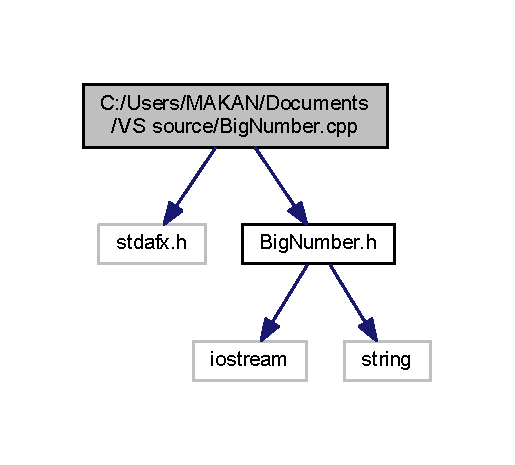
\includegraphics[width=247pt]{_big_number_8cpp__incl}
\end{center}
\end{figure}

\hypertarget{_big_number_8h}{}\section{C\+:/\+Users/\+M\+A\+K\+A\+N/\+Documents/\+VS source/\+Big\+Number.h File Reference}
\label{_big_number_8h}\index{C\+:/\+Users/\+M\+A\+K\+A\+N/\+Documents/\+V\+S source/\+Big\+Number.\+h@{C\+:/\+Users/\+M\+A\+K\+A\+N/\+Documents/\+V\+S source/\+Big\+Number.\+h}}


\mbox{\hyperlink{class_big_number}{Big\+Number}} class declarations.  


{\ttfamily \#include $<$iostream$>$}\newline
{\ttfamily \#include $<$string$>$}\newline
Include dependency graph for Big\+Number.\+h\+:\nopagebreak
\begin{figure}[H]
\begin{center}
\leavevmode
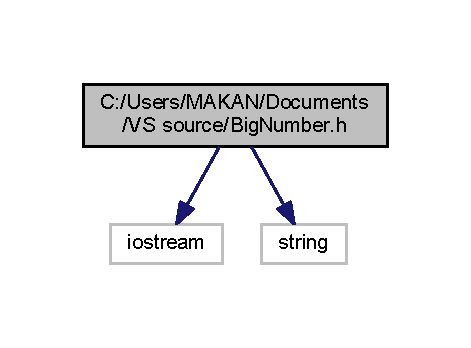
\includegraphics[width=226pt]{_big_number_8h__incl}
\end{center}
\end{figure}
This graph shows which files directly or indirectly include this file\+:\nopagebreak
\begin{figure}[H]
\begin{center}
\leavevmode
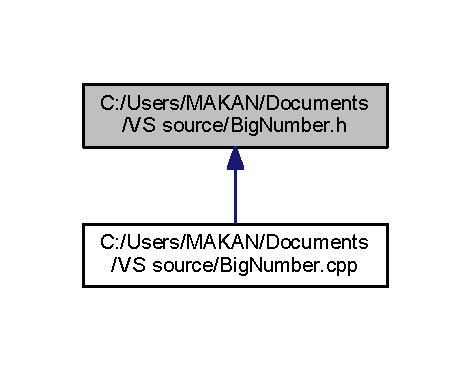
\includegraphics[width=226pt]{_big_number_8h__dep__incl}
\end{center}
\end{figure}
\subsection*{Classes}
\begin{DoxyCompactItemize}
\item 
class \mbox{\hyperlink{class_big_number}{Big\+Number}}
\end{DoxyCompactItemize}


\subsection{Detailed Description}
\mbox{\hyperlink{class_big_number}{Big\+Number}} class declarations. 


%--- End generated contents ---

% Index
\backmatter
\newpage
\phantomsection
\clearemptydoublepage
\addcontentsline{toc}{chapter}{Index}
\printindex

\end{document}
